%!TEX root = ../thesis.tex
%*******************************************************************************
%****************************** Third Chapter **********************************
%*******************************************************************************
\chapter{Predicting \mtb{} drug resistance}
\label{chap:dst}
% **************************** Define Graphics Path **************************
\ifpdf
    \graphicspath{{Chapter3/Figs/Raster/}{Chapter3/Figs/PDF/}{Chapter3/Figs/}}
\else
    \graphicspath{{Chapter3/Figs/Vector/}{Chapter3/Figs/}}
\fi

%=========================================================================
%=========================================================================

\setcounter{section}{-1}
\section{Publication and collaboration acknowledgements}
\label{sec:ch3-acknowledge}

A manuscript comprising the work in this chapter and \autoref{chap:clustering} is currently in preparation. In addition to the acknowledgements in \autoref{sec:ch2-acknowledge} the work not completed by myself in this chapter was the drug susceptibility testing (DST) in the laboratory.

\todo[inline]{need to confirm all of this with collabs once I have received the text outlining the methods}

The DST for the samples from Madagascar was conducted by Marie Sylvianne Rabodoarivelo and Simon Grandjean Lapierre. 

\towrite[inline]{acknowledge the people who did the south african DST}

\towrite[inline]{acknowledge the people who did the birmingham DST}


While I did all bioinformatic work in this chapter, I must acknowledge the excellent guidance I have received. My supervisor Zamin Iqbal who always knows the right questions to ask. Simon Grandjean Lapierre helped conceive of this study, along with Zam, and whose clinical perspective helped keep me grounded in the real world. I would also like to acknowledge the many insightful conversations with our other collaborators: Marie Sylvianne Rabodoarivelo, Anastasia Koch, Niaina Rakotosamimanana, Anzaan Dippenaar, and Helen Cox. 

%=========================================================================
\section{Introduction}

The software package Mykrobe provides antimicrobial resistance (AMR) predictions for \mtb{} - amongst other species. 
% talk about why the popn ref graph approach from mykrobe is lacking
Culture-based drug susceptibility testing is still considered the gold-standard for determining the phenotype of a sample.

Whilst the drug resistance prediction of mykrobehas been thoroughly evaluated for Illumina sequencing data, it has only been validated on 5 Nanopore samples (Hunt 2019). As our dataset does not have DST information for all samples, or even for all of the 11 drugs mykrobe provides predictions for, we aim to investigate the concordance of Nanopore and Illumina predictions. 

%=========================================================================
\section{Dataset}
% refer to previous chapter for sequencing info and mention we use the samples that passed QC
The \mtb{} samples used in this chapter are those described in \autoref{sec:ch2-dataset}. We use the 150 samples that passed quality control (\autoref{sec:ch2-qc}).

\subsection{Drug susceptibility testing}
\label{sec:dst-methods}
% I have asked the collaborators for the DST methods
\towrite[inline]{waiting for text from collaborators}

\noindent
In total, 128 samples have phenotypic information for at least one drug, with 80 having phenotypes for eight drugs. \autoref{tab:available-dst} shows the number of samples with culture-based DST for each drug and \autoref{fig:available-dst} depicts the combinations of drugs available for samples. For instance, in \autoref{fig:available-dst}, the third column reveals that 29 samples have phenotype information for ofloxacin and amikacin, while row three shows that 51 samples have available DST for kanamycin. 

Although line probe assays (LPAs) were also completed for many samples, we base our analysis of concordance with phenotype on the culture-based DST data. However, we do use the LPA information to inform reasons for possible errors with drug prediction. \autoref{tab:full-dst} and \autoref{fig:full-dst} in \autoref{sec:full-dst} shows the full available DST data from both culture-based and LPA methods.

\begin{table}
\centering
\begin{tabular}{|l|c|}
\hline
Drug         & Count \\ \hline
Amikacin     & 88    \\ \hline
Capreomycin  & 51    \\ \hline
Ethambutol   & 90    \\ \hline
Isoniazid    & 98    \\ \hline
Kanamycin    & 51    \\ \hline
Moxifloxacin & 1     \\ \hline
Ofloxacin    & 86    \\ \hline
Pyrazinamide & 1     \\ \hline
Rifampicin   & 91    \\ \hline
Streptomycin & 90    \\ \hline
\end{tabular}
\caption{Culture-based drug susceptibility data available for samples. The counts are the number of samples with phenotype information available for that drug.}
\label{tab:available-dst}
\end{table}

\begin{figure}
\begin{center}
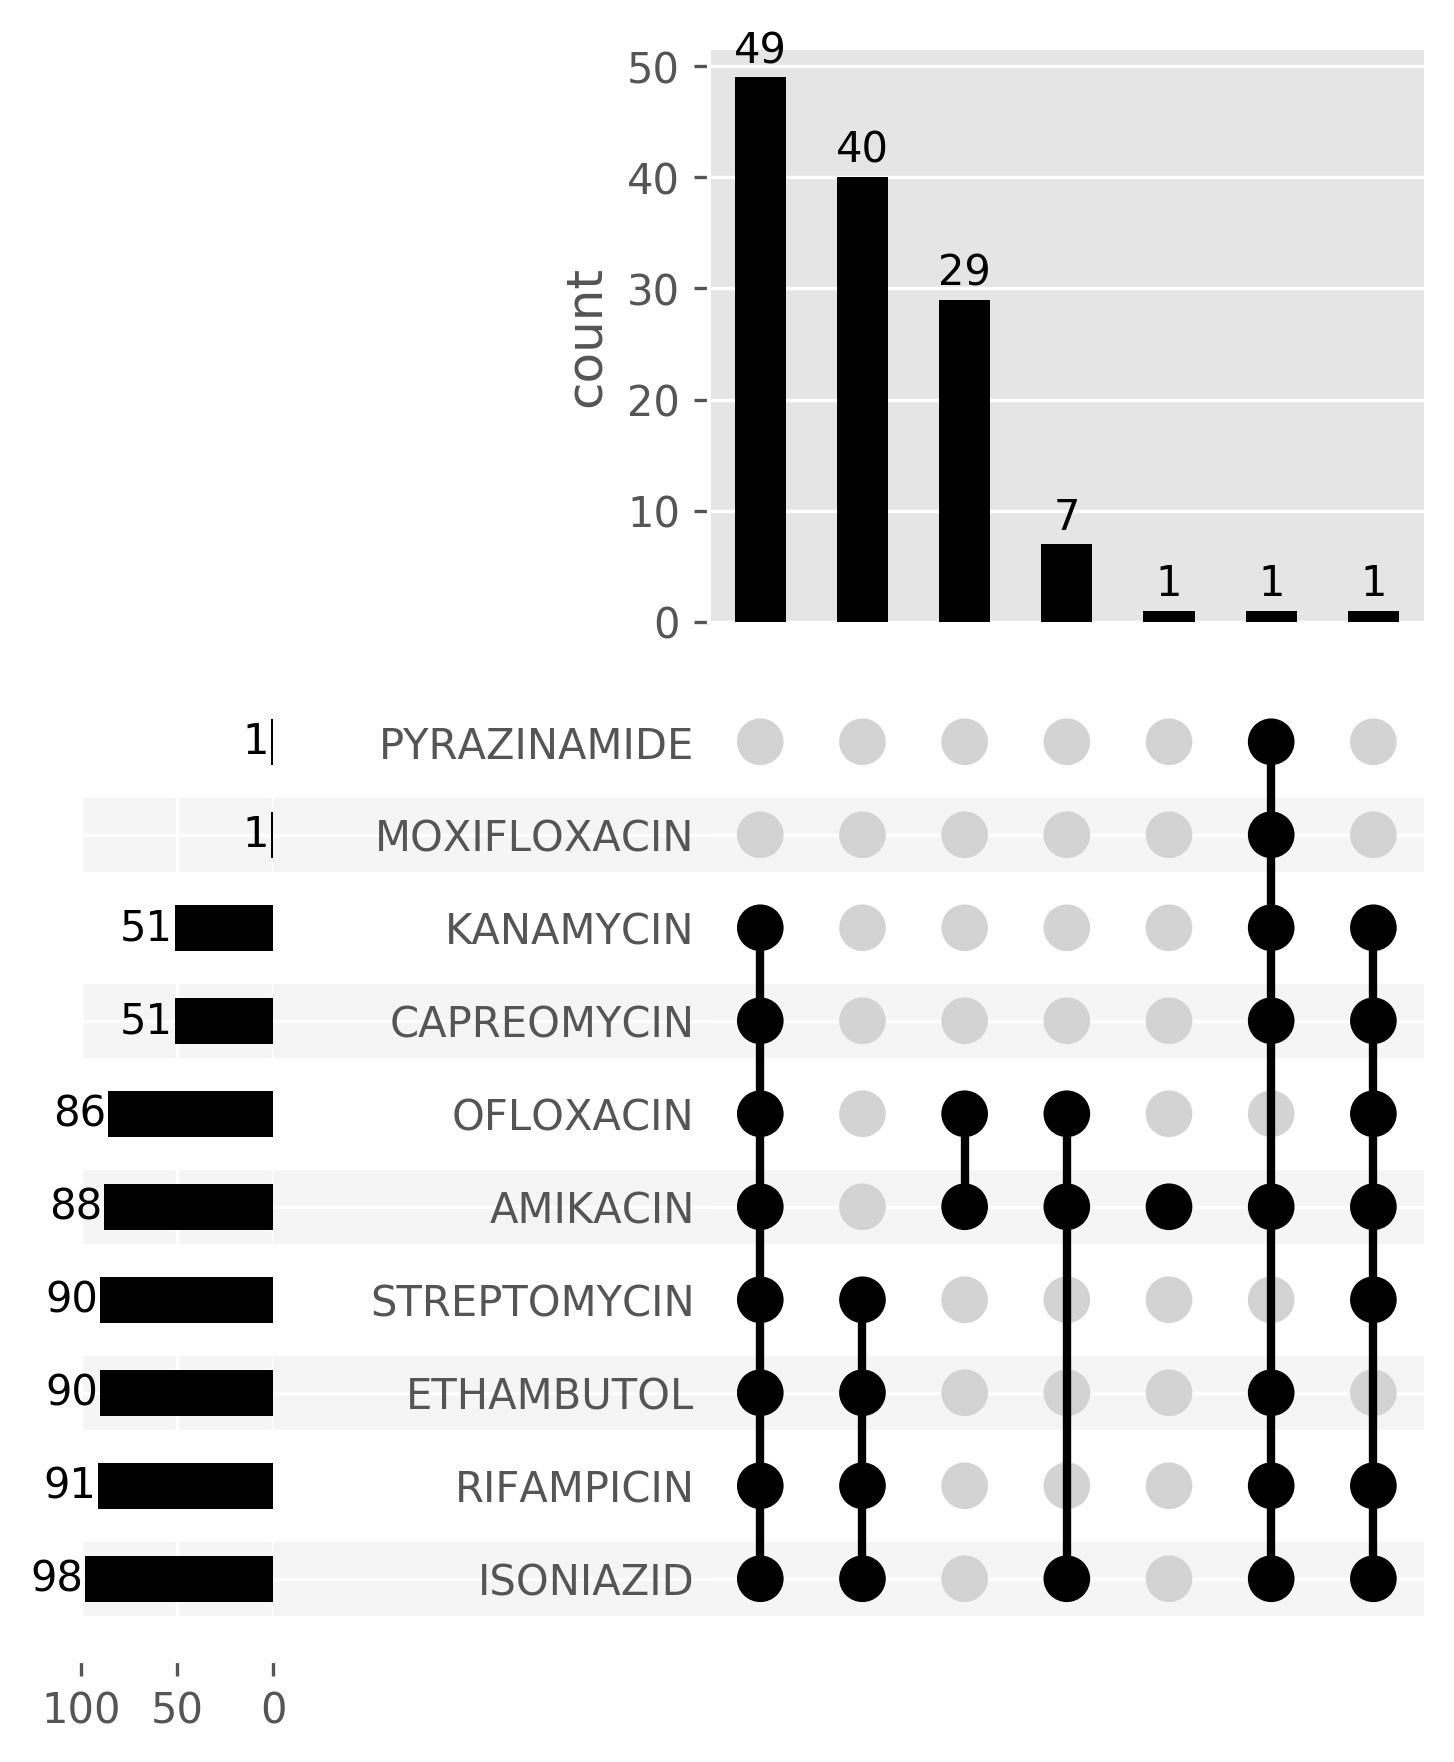
\includegraphics[width=0.90\columnwidth]{Chapter3/Figs/available_dst.png}
\caption{{Culture-based drug susceptibility data available for samples. Each row is a drug, and the columns represent a set of samples that have phenotype information for those drugs with a filled cell. The top panel shows the number of samples in the set for that combination of drugs. The bar plot in the left panel shows the number of samples with phenotype information for that drug.
{\label{fig:available-dst}}
}}
\end{center}
\end{figure}
%=========================================================================
\section{Drug resistance prediction with genome graphs}
\label{sec:drprg-methods}
% i.e., methods for drprg
In this section, we set out to design a software program that uses genome graphs to predict drug resistance for \mtb{}; building on previous work in this thesis building \mtb{} \prg{}s (\autoref{sec:tbprg}) and calling variants (\autoref{sec:pandora-filters} and \autoref{chap:denovo}). The tool we developed, \drprg{} (Drug Resistance Prediction with Reference Graphs), is written in the Rust programming language and can be found at \url{https://github.com/mbhall88/drprg}.
% some of this might be better off in the intro
While tools already exist for the purpose of prediction AMR, the unique component of \drprg{} is the ability to call novel variants. As the \cryptic{} Consortium recently showed, refusing to predict drug phenotypes in cases where "unknown" mutations are present in the associated target gene can lead to increased detection of pan-susceptibility for first-line drugs \cite{cryptic2018}. However, no tool usable by others made available in that work, and reproducing the results requires running multiple separate tools and scripts. \drprg{} offers a single point for producing this information.

\drprg{} has two distinct phases. In the first phase, an index and \prg{} are built from a panel of variants known to cause resistance or susceptibility. Second, Illumina or \ont{} reads are provided and phenotype predictions are made for the drugs in the provided panel.

We now outline these two steps in detail.

\subsection{Constructing a panel reference graph}
\label{sec:drprg-index}
The first stage of predicting drug resistance from \drprg{} is coordinated by the \vrb{build} subcommand. As input, \vrb{build} requires a panel of variants, and a reference genome and annotation. We use the reference and annotation (GFF) for the \mtb{} strain H37Rv (accession NC\_000962.3) and the default panel used by mykrobe (v0.10.0) \cite{hunt2019}. 

The panel of variants can be either resistance- or susceptibility-associated. Each entry in the panel file describes, the gene the variant occurs in and the mutation it causes. The mutation can represent a DNA or protein change and is given in the form reference, position, alternate. For example a DNA mutation, \vrb{A5T}, indicates the reference base, \vrb{A}, at position 5 in the gene, is changed to a \vrb{T}. An \vrb{X} is used to indicate any nucleic or amino acid other than the one listed as the reference. If a variant is resistance-associated, a list of drugs must also be given, otherwise, if "NONE" is given, the variant is assumed not be associated with resistance.

After the panel has been loaded, for each gene listed, we generate a reference sequence using the provided reference genome and annotation. If the optional padding argument is given, we add the provided number of bases to the start and end of each gene reference sequence - we used padding of 100bp.

The next step is to convert the panel into a VCF representation. For protein mutations, we convert the amino acids into their respective DNA forms (all possible codons). We confirm the reference codon matches the reference sequence at the given position in the gene reference sequence. Positions for proteins are carefully converted to nucleic acid-space, taking into account the strand of transcription specified in the annotation. DNA mutations are likewise checked against the reference. A VCF entry is then generated for each panel entry using the DNA representation. For protein mutations and DNA mutations with an alternate of \vrb{X}, all possible alternates are listed in the same entry. An example panel and associated VCF can be seen in \autoref{fig:example-panel}.

Another optional parameter of \drprg{} \vrb{build} is the ability to provide a prebuilt \prg{}. If no prebuilt \prg{} is provided, \drprg{} will construct one from the panel. It does this in a similar fashion to the method described in \autoref{sec:tbprg}. That is, for each VCF entry and alternate allele, we replace the gene reference position(s) with the alternate, and combine all such mutated sequences into a single FASTA file. We perform a multiple sequence alignment (MSA) on each file, followed by converting the MSA into a local \prg{} using \makeprg{}. Finally, the resulting local \prg{}s, which represent each gene in the panel, are combined into a single \prg{} and indexed with \pandora{}.

For the work in this chapter, we chose to use a prebuilt, population-based \prg{}, rather than the panel \prg{} constructed by \drprg{}. In the early stages of testing and developing \drprg{} we found the panel-based \prg{} density and lack of haplotype information was causing a lot of missed resistance (false negatives). \autoref{app:panel-prg-issues} provides a thorough investigation into these problems with the panel-based \prg{}.

The population-based \prg{} we use is built from the same variants as the sparse \prg{} in \autoref{sec:tbprg} - with an important difference. In \autoref{sec:improve-prg} we discussed a potential improvement for the \prg{} construction process whereby whole haplotypes are applied to a reference sequence. When we constructed the original sparse \prg{} in \autoref{sec:tbprg}, we applied each variant \emph{in isolation} to the reference sequence. So, if a sample had 3 variants, we built the \prg{} from the reference sequence, plus 3 mutated versions of that reference (see \autoref{sec:improve-prg} for a detailed example). Instead, for the \prg{} we use in this chapter, we apply \emph{all} variants for a sample in the sparse VCF to the (gene) reference sequence - producing a single (gene) haplotype sequence for that sample. We do this for all genes, and use the same MSA, \makeprg{}, \pandora{} index approach mentioned above (and in \autoref{sec:tbprg}). One major difference being the use of a \makeprg{} prototype (v0.2 - mentioned in \autoref{sec:fw-comp-perf}) with a minimum match length of 5. This prototype, developed by Leandro Ishi, retains information about the clustering of sites for each local \prg{}, allowing for quicker updating of \prg{}s with novel variants (as discussed in \autoref{sec:drprg-predict}).


\subsection{Predictions}
\label{sec:drprg-predict}
% how we go from reads and panel to predictions
% also outline what we do with novel stuff
The second, and final stage of predicting drug resistance with \drprg{} is the the \vrb{predict} routine. It takes an index produced by \drprg{} \vrb{build} (\autoref{sec:drprg-index}) and a file containing sequencing reads (Illumina or \ont{}). One optional parameter of interest for the work in this chapter is the ability to discover novel variants.

If requested, the first stage of \drprg{} \vrb{predict} is novel variant discovery in the sequencing reads with \pandora{} \vrb{discover} (using version 0.9.0). This version of \pandora{} differs to the one used in \autoref{chap:clustering} in that it outputs all novel variants into a single file compatible with the \makeprg{} prototype used in \autoref{sec:drprg-index}. Next, \makeprg{} updates the \drprg{} \prg{} with these new variants and the resulting updated \prg{} is indexed with \pandora{}. 

One downside to using a population-based \prg{} as we do, is that unlike the panel-based \prg{}, it does not contain all panel variants. As such, for the work in this chapter, we request novel variant discovery in \drprg{} \vrb{predict}.

The second step of \vrb{predict} is genotyping of the sample's sequencing data against the \prg{} (updated or original depending on if variant discovery is requested) with \pandora{} \vrb{map}. An important part of the genotyping step is that we force \pandora{} to output variant coordinated with respect to the gene reference sequences in the index from \vrb{build} using the \vrb{--vcf-refs} argument. That way, the resulting genotyped VCF coordinates can be compared to the panel VCF in the index. 

After producing the \pandora{} genotyped VCF, we filter out variants that do not meet the provided filtering criteria. \drprg{} \vrb{predict} allows filtering based on minimum and maximum read depth, strand bias, minimum genotype confidence, minimum fraction of read support (FRS), and maximum indel size (see \autoref{sec:pandora-filters} for more information on these fields). For the results presented in this chapter, we use a minimum read depth of 3, a minimum FRS of 70\%, a minimum genotype confidence score of 5, a maximum indel size of 20, and a minimum strand bias of 1\% (i.e, we require at least 1\% of total read coverage on both strands). If a variant fails any of these filters, it is ignored from subsequent analysis.

Next, we make resistance predictions from the variants that pass filtering (calls). For each call in the (filtered) genotyped VCF, we fetch all panel variants (from the panel VCF) that have overlapping coordinates. If there are no panel variants that overlap the call, and novel variant discovery was requested, we classify all drugs with resistance-causing mutations in the gene the call was made in as "unknown" ('U') - otherwise we skip the call. If the call is a null genotype (\vrb{.}), we predict all overlapping panel variants as "failed" (denoted by 'F').

If the variant call was not deemed unknown or failed in the previous step, and it has overlapping panel variants, we check if there is a match between the call and a panel allele. To determine whether a match exists, we iterate through each of the panel alleles (including the reference) and extract overlapping sequence between it and the called sequence. If the panel and called allele start at the same position, this is as simple as trimming both sequences to the length of the shortest of the two (if they aren't the same length). In the case where they start at different positions, we extract the subsequence denoted by the intersection between the two allele's intervals. For example, if the called allele, \vrb{AT}, starts at position 4 and the panel allele, \vrb{TG}, starts at position 5, their (half-open) intervals are $[4,6)$ and $[5,7)$ respectively. The intersection of these two intervals would be $[5,6)$ which yields a subsequence of \vrb{T} for both, and thus we would deem the two a match. When the two alleles do not have the same length - e.g., indels - we additionally track the length of the matching sequences relative to the reference allele. That way, when there is more than one panel allele that matches the called allele, we return the allele with the match whose length is closest to the called allele.

We add two annotations to each of the genotyped VCF entries that overlap variants in the panel: \vrb{VARID} and \vrb{PREDICT}. \vrb{VARID} is a list of panel variants the position overlaps and \vrb{PREDICT} is a prediction for each of those panel variants. If there was a non-reference match between a panel variant and the called allele, and the panel variant is resistance-causing, a prediction of resistant is recorded. If there was no match, and variant discovery was requested, a prediction of unknown is given, otherwise it is deemed susceptible. 

After adding the prediction annotations to each entry in the genotyped VCF, we produce a final prediction report as a JSON file. A prediction is provided for every drug present in the panel, along with the evidence (variant(s)) that supports the prediction. We generate these predictions by going back through the genotyped VCF and using the \vrb{PREDICT} annotation added in the previous step. When different predictions are present for the same drug, the precedence, in order, is resistant, unknown, failed, and susceptible. An example report can be seen in \autoref{fig:example-drprg-report}.

\noindent
All \drprg{} results in this chapter were generated using the commit \href{https://github.com/mbhall88/drprg/tree/cb4f9b82b5d03de45b8016ae5d54bbce7a8f3a0f}{\vrb{cb4f9b8}}.

\subsection{Computational performance}

We compare the peak memory usage and runtime for \drprg{} \vrb{predict} with the other tool used for resistance prediction in this chapter, mykrobe. \autoref{fig:predict-comp-perf} shows the computational performance of both tools, split by sequencing technology. On average, \drprg{} is faster than mykrobe for both Illumina and Nanopore and uses less memory. As summarised in \autoref{tab:predict-comp-pref}, \drprg{} has a median CPU time of 11.84s (Illumina) and 178.41s (\ont{}) compared to mykrobe's 196.90s (Illumina) and 248.81s (\ont{}). In terms of memory usage, \drprg{} had a median peak of 224MB (Illumina) and 345.50MB (\ont{}) compared with mykrobe's 1193.00MB (Illumina) and 1195.00MB (\ont{}). However, for both tools, these time and memory figures are more than sufficient to comfortably run either tool on a standard laptop. 

Building the \drprg{} population-based \prg{} and index took 174.53s of CPU time in total and had a peak memory usage of 368MB, which occurred during the \makeprg{} step.

\begin{figure}
\begin{center}
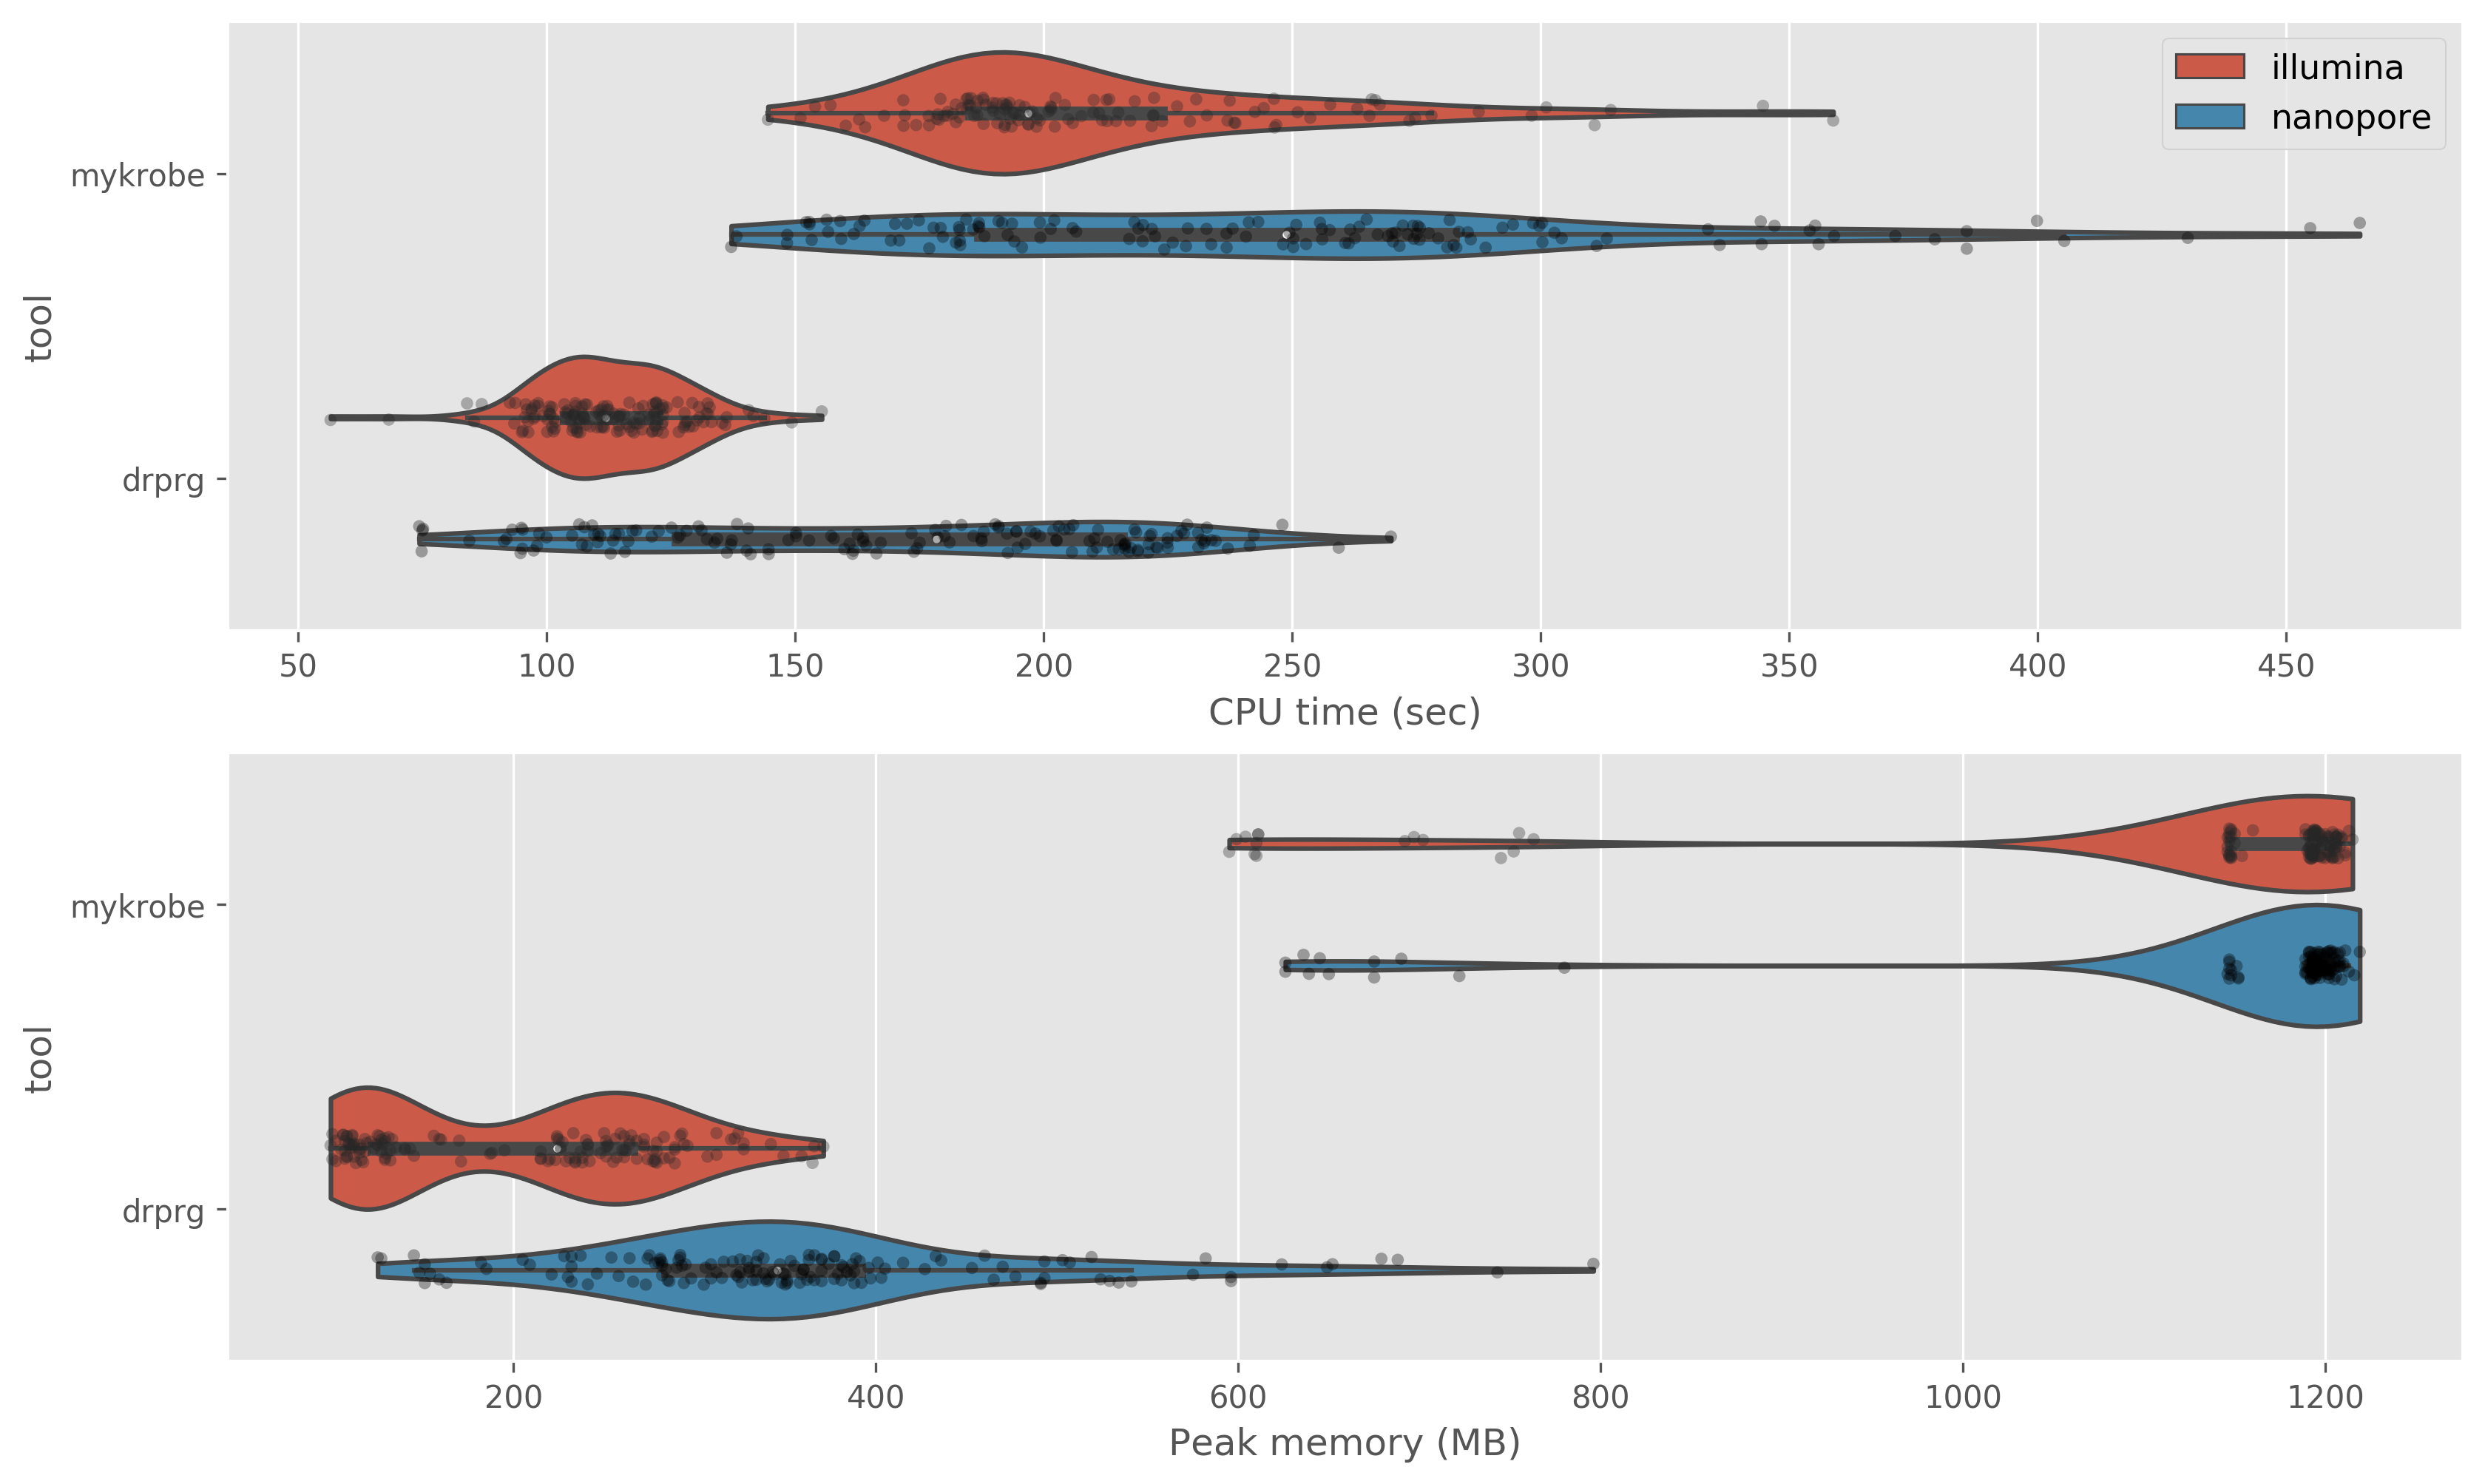
\includegraphics[width=0.90\columnwidth]{Chapter3/Figs/predict-comp-perf.png}
\caption{{The time (seconds; top) and memory (megabytes; bottom) usage of mykrobe and \drprg{} for generating drug resistance predictions. Each tool is additionally split into sequencing technology, with Illumina in red and \ont{} in blue. Data points indicate individual results for a single sample.
{\label{fig:predict-comp-perf}}
}}
\end{center}
\end{figure}


\begin{table}
\centering
\begin{tabular}{|l|l|r|r|r|r|}
\hline
\multicolumn{2}{|l|}{tool}       & \multicolumn{2}{l|}{\drprg{}} & \multicolumn{2}{l|}{mykrobe} \\ \hline
\multicolumn{2}{|l|}{technology} & illumina     & nanopore    & illumina      & nanopore     \\ \hline
\multirow{7}{*}{time (s)}    & mean  & 112.85       & 170.06      & 209.71        & 247.75       \\ \cline{2-6} 
                         & std   & 14.37        & 49.28       & 38.59         & 69.85        \\ \cline{2-6} 
                         & min   & 56.51        & 74.34       & 144.51        & 137.11       \\ \cline{2-6} 
                         & 25\%  & 103.95       & 126.50      & 185.55        & 187.29       \\ \cline{2-6} 
                         & 50\%  & 111.84       & 178.41      & 196.90        & 248.81       \\ \cline{2-6} 
                         & 75\%  & 122.05       & 215.37      & 223.41        & 282.25       \\ \cline{2-6} 
                         & max   & 155.34       & 269.84      & 358.83        & 464.77       \\ \hline
\multirow{7}{*}{memory (MB)}  & mean  & 203.28       & 357.47      & 1126.33       & 1151.14      \\ \cline{2-6} 
                         & std   & 78.64        & 121.38      & 173.29        & 145.87       \\ \cline{2-6} 
                         & min   & 99.00        & 125.00      & 595.00        & 626.00       \\ \cline{2-6} 
                         & 25\%  & 123.25       & 285.25      & 1148.50       & 1192.00      \\ \cline{2-6} 
                         & 50\%  & 224.00       & 345.50      & 1193.00       & 1195.00      \\ \cline{2-6} 
                         & 75\%  & 264.75       & 390.50      & 1201.00       & 1201.00      \\ \cline{2-6} 
                         & max   & 371.00       & 796.00      & 1215.00       & 1219.00      \\ \hline
\end{tabular}
\caption{Summary statistics for the CPU time and peak memory usage of drug resistance prediction with mykrobe and \drprg{} for Illumina and \ont{} data. std=standard deviation}
\label{tab:predict-comp-pref}
\end{table}

%=========================================================================
\section{Genotypic resistance prediction concordance with phenotype}
\label{sec:pheno-concordance}

In this section we aim to assess the capability of \ont{} WGS, and the genome graph-based approach - \drprg{} - outlined in \autoref{sec:drprg-methods}, to provide reliable drug resistance predictions.

The culture-based DST profiles gathered in \autoref{sec:dst-methods}, where available, are considered the true phenotype against which we will appraise the WGS methods. We exclude moxifloxacin and pyrazinamide from this phenotype concordance analysis as DST was only performed for one sample (see \autoref{tab:available-dst}). The total number of samples with cultured-based DST information for each drug are outlined in \autoref{tab:available-dst}.

We compare the WGS-based drug resistance predictions from mykrobe (version 0.10.0; \cite{hunt2019}) and \drprg{} for both Illumina and \ont{} data. For the predictions from mykrobe, some default settings were altered as a result of the analysis in \autoref{app:mykrobe-settings}. The Illumina expected error rate was decreased from 0.05 (default) to 0.001, while the preset \ont{} settings were disabled in favour of an expected error rate of 0.08 and disabling minor resistance calls (haploid model). The \drprg{} settings are detailed in \autoref{sec:drprg-predict}. 

For the drug/sample combinations with available culture-based phenotypes, we classify the WGS predictions as follows. True positive (TP) when the prediction and phenotype are both resistant; true negative (TN) when the prediction and phenotype are both susceptible; false positive (FP) when the prediction is resistant but the phenotype is susceptible; false negative (FN) when the prediction is susceptible but the phenotype is resistant. For this phenotype concordance analysis we ignore failed and unknown resistance calls from \drprg{} and consider them as susceptible (we assess the utility of these features in \autoref{sec:drprg-discover}). Additionally, for mykrobe Illumina predictions, we interpret minor resistance calls (`r') as resistance (`R').

\autoref{fig:pheno-concordance} shows the concordance of WGS predictions with culture-based phenotypes. The left panel illustrates the number of correct and missed resistance calls made by mykrobe and \drprg{} for both Illumina and \ont{} data. In the right panel, we show the number of correct and incorrect susceptibility predictions. \autoref{tab:pheno-concordance} provides the number of FNs and FPs, along with the false negative rate, false positive rate, positive predictive value, and negative predictive value for each technology/drug combination. 

These results provide a positive outcome for both our aims. First, \ont{} predictions (striped bars in \autoref{sec:pheno-concordance}) are highly congruent with Illumina. That is, they have equivalent numbers for each classification category. One exception to this is mykrobe \ont{} having noticeably more FPs for isoniazid compared with its Illumina equivalent; all the extra FP calls were related to an indel with no Illumina support. Second, the genome graph-based approach \drprg{}, developed in this chapter, provides predictions consistent with mykrobe - and in some cases slightly better. 

Ethambutol and streptomycin had a large number of FPs compared to the other drugs for both prediction tools. On further investigation, all ethambutol FPs contain strong evidence for a non-synonymous mutation at codon 306 in \textit{embB}, which is known to be strongly linked to drug resistance \cite{Maningi2017,Srivastava2009,Brossier2015}. Of the 14 (16 for mykrobe Illumina) samples with FP ethambutol calls, six additionally had LPA phenotypes and in all cases the LPA disagreed with the culture-based phenotype (i.e., LPA was resistant and culture was susceptible). Taken together, this information would suggest the culture-based phenotype may be wrong.

While there is no LPA data for streptomycin to check discrepancies, an interesting observation is that 23/38 (60\%) of ethambutol FPs also had a FP streptomycin prediction. There was no one particular mutation found amongst the streptomycin FPs, but in all cases the predicted variant had very strong support from the tool and the relevant COMPASS and \bcftools{} VCFs from \autoref{sec:var-calls}.

Isoniazid FNs...


\begin{figure}
\begin{center}
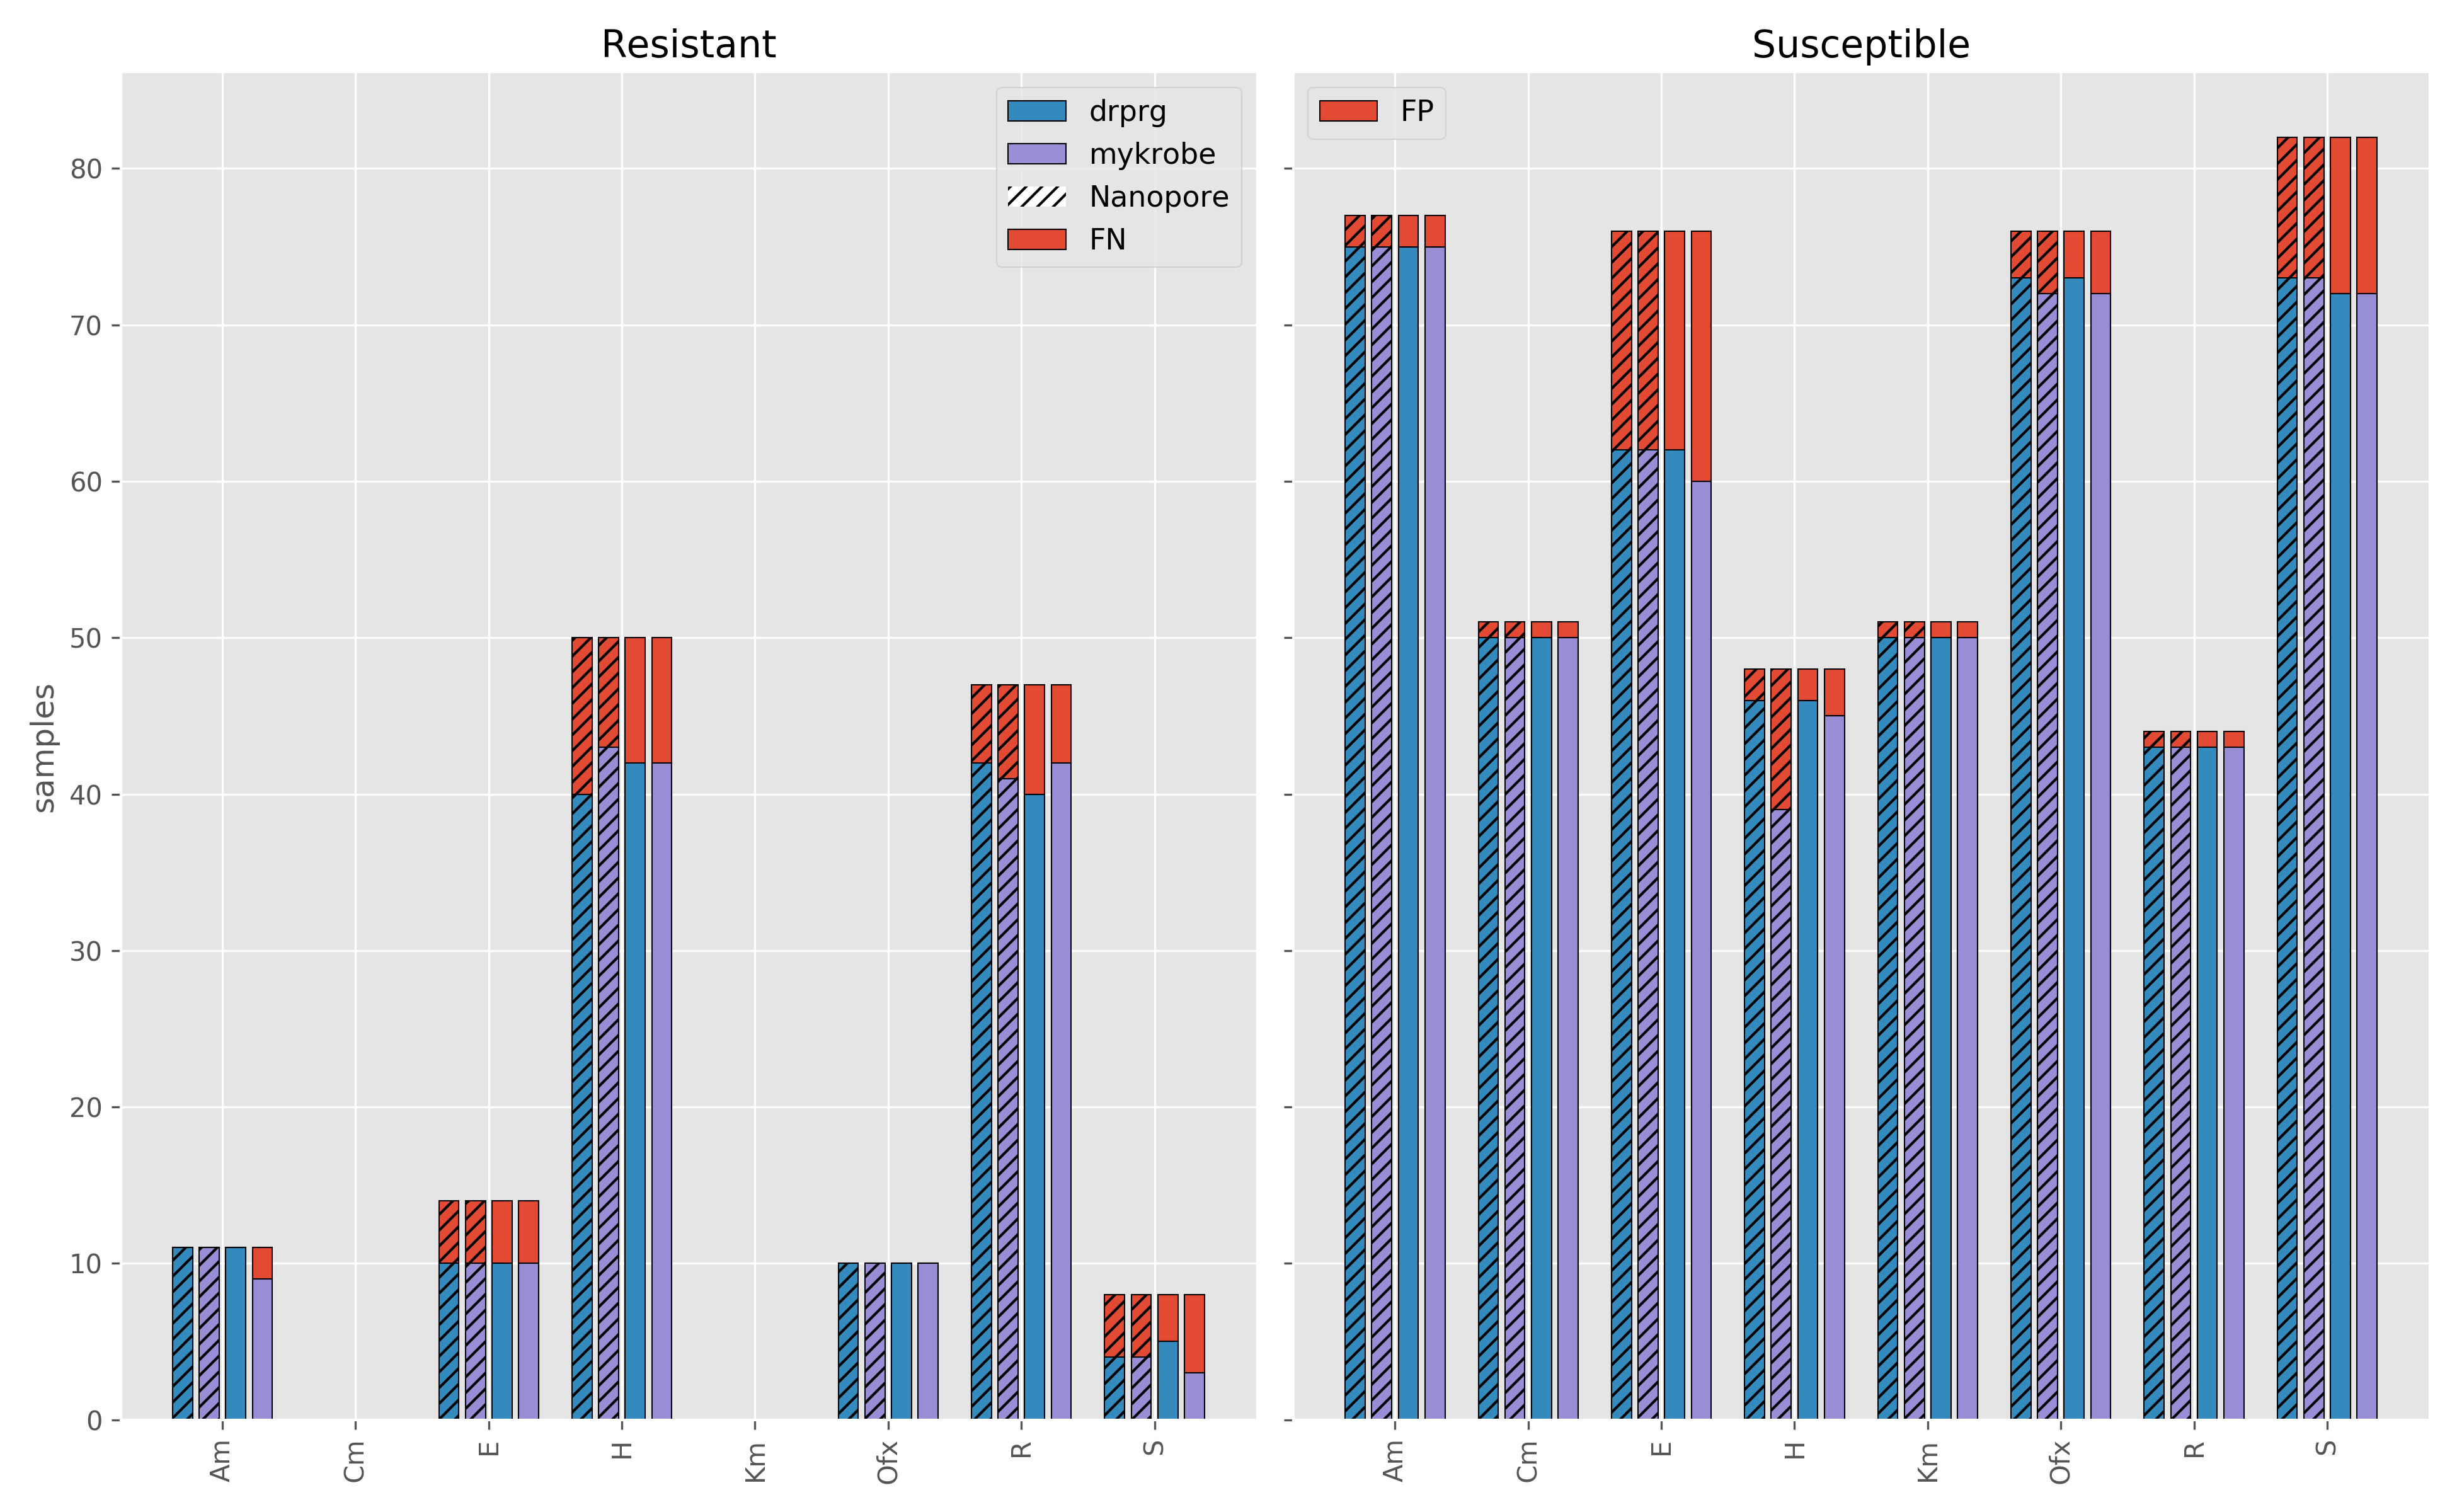
\includegraphics[width=0.90\columnwidth]{Chapter3/Figs/pheno_concordance_plot.png}
\caption{{Number of resistant (left) and susceptible (right) phenotypes correctly identified by mykrobe from Illumina (blue) and Nanopore (purple) data from the same samples. The red bars indicate missed (FN) or incorrect (FP) predictions. The x-axis shows the drugs with available phenotype data that mykrobe also makes predictions for. E - ethambutol; H - isoniazid; Z - pyrazinamide; R - rifampicin; S - streptomycin; Km - kanamycin; Am - amikacin; Ofx - ofloxacin; Cm - capreomycin; Mfx - moxifloxacin.
{\label{fig:pheno-concordance}}
}}
\end{center}
\end{figure}

% Please add the following required packages to your document preamble:
% \usepackage{multirow}
% \usepackage{graphicx}
\begin{table}
\centering
\resizebox{\textwidth}{!}{%
\begin{tabular}{|l|l|l|l|l|l|l|l|l|}
\hline
Drug &
  Technology &
  Tool &
  FN(R) &
  FP(S) &
  FNR(95\% CI) &
  FPR(95\% CI) &
  PPV(95\% CI) &
  NPV(95\% CI) \\ \hline
\multirow{4}{*}{Amikacin} &
  \multirow{2}{*}{Illumina} &
  Drprg &
  0(11) &
  2(77) &
  0.0\% (0.0-25.9\%) &
  2.6\% (0.7-9.0\%) &
  84.6\% (57.8-95.7\%) &
  100.0\% (95.1-100.0\%) \\ \cline{3-9} 
 &
   &
  Mykrobe &
  2(11) &
  2(77) &
  18.2\% (5.1-47.7\%) &
  2.6\% (0.7-9.0\%) &
  81.8\% (52.3-94.9\%) &
  97.4\% (91.0-99.3\%) \\ \cline{2-9} 
 &
  \multirow{2}{*}{Nanopore} &
  Drprg &
  0(11) &
  2(77) &
  0.0\% (0.0-25.9\%) &
  2.6\% (0.7-9.0\%) &
  84.6\% (57.8-95.7\%) &
  100.0\% (95.1-100.0\%) \\ \cline{3-9} 
 &
   &
  Mykrobe &
  0(11) &
  2(77) &
  0.0\% (0.0-25.9\%) &
  2.6\% (0.7-9.0\%) &
  84.6\% (57.8-95.7\%) &
  100.0\% (95.1-100.0\%) \\ \hline
\multirow{4}{*}{Capreomycin} &
  \multirow{2}{*}{Illumina} &
  Drprg &
  0(0) &
  1(51) &
  - &
  2.0\% (0.3-10.3\%) &
  0.0\% (0.0-79.3\%) &
  100.0\% (92.9-100.0\%) \\ \cline{3-9} 
 &
   &
  Mykrobe &
  0(0) &
  1(51) &
  - &
  2.0\% (0.3-10.3\%) &
  0.0\% (0.0-79.3\%) &
  100.0\% (92.9-100.0\%) \\ \cline{2-9} 
 &
  \multirow{2}{*}{Nanopore} &
  Drprg &
  0(0) &
  1(51) &
  - &
  2.0\% (0.3-10.3\%) &
  0.0\% (0.0-79.3\%) &
  100.0\% (92.9-100.0\%) \\ \cline{3-9} 
 &
   &
  Mykrobe &
  0(0) &
  1(51) &
  - &
  2.0\% (0.3-10.3\%) &
  0.0\% (0.0-79.3\%) &
  100.0\% (92.9-100.0\%) \\ \hline
\multirow{4}{*}{Ethambutol} &
  \multirow{2}{*}{Illumina} &
  Drprg &
  4(14) &
  14(76) &
  28.6\% (11.7-54.6\%) &
  18.4\% (11.3-28.6\%) &
  41.7\% (24.5-61.2\%) &
  93.9\% (85.4-97.6\%) \\ \cline{3-9} 
 &
   &
  Mykrobe &
  4(14) &
  16(76) &
  28.6\% (11.7-54.6\%) &
  21.1\% (13.4-31.5\%) &
  38.5\% (22.4-57.5\%) &
  93.8\% (85.0-97.5\%) \\ \cline{2-9} 
 &
  \multirow{2}{*}{Nanopore} &
  Drprg &
  4(14) &
  14(76) &
  28.6\% (11.7-54.6\%) &
  18.4\% (11.3-28.6\%) &
  41.7\% (24.5-61.2\%) &
  93.9\% (85.4-97.6\%) \\ \cline{3-9} 
 &
   &
  Mykrobe &
  4(14) &
  14(76) &
  28.6\% (11.7-54.6\%) &
  18.4\% (11.3-28.6\%) &
  41.7\% (24.5-61.2\%) &
  93.9\% (85.4-97.6\%) \\ \hline
\multirow{4}{*}{Isoniazid} &
  \multirow{2}{*}{Illumina} &
  Drprg &
  8(50) &
  2(48) &
  16.0\% (8.3-28.5\%) &
  4.2\% (1.2-14.0\%) &
  95.5\% (84.9-98.7\%) &
  85.2\% (73.4-92.3\%) \\ \cline{3-9} 
 &
   &
  Mykrobe &
  8(50) &
  3(48) &
  16.0\% (8.3-28.5\%) &
  6.2\% (2.1-16.8\%) &
  93.3\% (82.1-97.7\%) &
  84.9\% (72.9-92.1\%) \\ \cline{2-9} 
 &
  \multirow{2}{*}{Nanopore} &
  Drprg &
  10(50) &
  2(48) &
  20.0\% (11.2-33.0\%) &
  4.2\% (1.2-14.0\%) &
  95.2\% (84.2-98.7\%) &
  82.1\% (70.2-90.0\%) \\ \cline{3-9} 
 &
   &
  Mykrobe &
  7(50) &
  9(48) &
  14.0\% (7.0-26.2\%) &
  18.8\% (10.2-31.9\%) &
  82.7\% (70.3-90.6\%) &
  84.8\% (71.8-92.4\%) \\ \hline
\multirow{4}{*}{Kanamycin} &
  \multirow{2}{*}{Illumina} &
  Drprg &
  0(0) &
  1(51) &
  - &
  2.0\% (0.3-10.3\%) &
  0.0\% (0.0-79.3\%) &
  100.0\% (92.9-100.0\%) \\ \cline{3-9} 
 &
   &
  Mykrobe &
  0(0) &
  1(51) &
  - &
  2.0\% (0.3-10.3\%) &
  0.0\% (0.0-79.3\%) &
  100.0\% (92.9-100.0\%) \\ \cline{2-9} 
 &
  \multirow{2}{*}{Nanopore} &
  Drprg &
  0(0) &
  1(51) &
  - &
  2.0\% (0.3-10.3\%) &
  0.0\% (0.0-79.3\%) &
  100.0\% (92.9-100.0\%) \\ \cline{3-9} 
 &
   &
  Mykrobe &
  0(0) &
  1(51) &
  - &
  2.0\% (0.3-10.3\%) &
  0.0\% (0.0-79.3\%) &
  100.0\% (92.9-100.0\%) \\ \hline
\multirow{4}{*}{Ofloxacin} &
  \multirow{2}{*}{Illumina} &
  Drprg &
  0(10) &
  3(76) &
  0.0\% (-0.0-27.8\%) &
  3.9\% (1.4-11.0\%) &
  76.9\% (49.7-91.8\%) &
  100.0\% (95.0-100.0\%) \\ \cline{3-9} 
 &
   &
  Mykrobe &
  0(10) &
  4(76) &
  0.0\% (-0.0-27.8\%) &
  5.3\% (2.1-12.8\%) &
  71.4\% (45.4-88.3\%) &
  100.0\% (94.9-100.0\%) \\ \cline{2-9} 
 &
  \multirow{2}{*}{Nanopore} &
  Drprg &
  0(10) &
  3(76) &
  0.0\% (-0.0-27.8\%) &
  3.9\% (1.4-11.0\%) &
  76.9\% (49.7-91.8\%) &
  100.0\% (95.0-100.0\%) \\ \cline{3-9} 
 &
   &
  Mykrobe &
  0(10) &
  4(76) &
  0.0\% (-0.0-27.8\%) &
  5.3\% (2.1-12.8\%) &
  71.4\% (45.4-88.3\%) &
  100.0\% (94.9-100.0\%) \\ \hline
\multirow{4}{*}{Rifampicin} &
  \multirow{2}{*}{Illumina} &
  Drprg &
  7(47) &
  1(44) &
  14.9\% (7.4-27.7\%) &
  2.3\% (0.4-11.8\%) &
  97.6\% (87.4-99.6\%) &
  86.0\% (73.8-93.0\%) \\ \cline{3-9} 
 &
   &
  Mykrobe &
  5(47) &
  1(44) &
  10.6\% (4.6-22.6\%) &
  2.3\% (0.4-11.8\%) &
  97.7\% (87.9-99.6\%) &
  89.6\% (77.8-95.5\%) \\ \cline{2-9} 
 &
  \multirow{2}{*}{Nanopore} &
  Drprg &
  5(47) &
  1(44) &
  10.6\% (4.6-22.6\%) &
  2.3\% (0.4-11.8\%) &
  97.7\% (87.9-99.6\%) &
  89.6\% (77.8-95.5\%) \\ \cline{3-9} 
 &
   &
  Mykrobe &
  6(47) &
  1(44) &
  12.8\% (6.0-25.2\%) &
  2.3\% (0.4-11.8\%) &
  97.6\% (87.7-99.6\%) &
  87.8\% (75.8-94.3\%) \\ \hline
\multirow{4}{*}{Streptomycin} &
  \multirow{2}{*}{Illumina} &
  Drprg &
  3(8) &
  10(82) &
  37.5\% (13.7-69.4\%) &
  12.2\% (6.8-21.0\%) &
  33.3\% (15.2-58.3\%) &
  96.0\% (88.9-98.6\%) \\ \cline{3-9} 
 &
   &
  Mykrobe &
  5(8) &
  10(82) &
  62.5\% (30.6-86.3\%) &
  12.2\% (6.8-21.0\%) &
  23.1\% (8.2-50.3\%) &
  93.5\% (85.7-97.2\%) \\ \cline{2-9} 
 &
  \multirow{2}{*}{Nanopore} &
  Drprg &
  4(8) &
  9(82) &
  50.0\% (21.5-78.5\%) &
  11.0\% (5.9-19.6\%) &
  30.8\% (12.7-57.6\%) &
  94.8\% (87.4-98.0\%) \\ \cline{3-9} 
 &
   &
  Mykrobe &
  4(8) &
  9(82) &
  50.0\% (21.5-78.5\%) &
  11.0\% (5.9-19.6\%) &
  30.8\% (12.7-57.6\%) &
  94.8\% (87.4-98.0\%) \\ \hline
\end{tabular}%
}
\caption{Comparison of drug resistance predictions with culture-based phenotype. For this comparison, we assume the drug susceptibility testing phenotype is correct and evaluate mykrobe Illumina and Nanopore resistance predictions accordingly. Pyrazinamide and Moxifloxacin are excluded as phenotype information is only available for 1 sample. FN=false negative; R=number of resistant samples; FP=false positive; S=number of susceptible samples; FNR=false negative rate; FPR=false positive rate; PPV=positive predictive value; NPV=negative predictive value; CI=Wilson score confidence interval}
\label{tab:pheno-concordance}
\end{table}
%=========================================================================
\section{Concordance with Illumina}
\label{sec:geno-concordance}
% ***************
% text from authorea
We saw in Section 3.5 that Nanopore-derived resistance predictions are inline with those from Illumina when comparing to DST information. As not all samples in the dataset have DST data, and not all samples with DST information have all drugs covered, we explore whether the Nanopore predictions are concordant with those from Illumina - for all drugs. As our sequencing data is matched, this analysis will highlight whether the prediction method used by mykrobe is well-tuned for Nanopore data. Given the rigorous and broad validation of mykrobe's prediction power on Illumina data, if Nanopore results are concordant, this will go a long way to endorsing it's use for resistance prediction.
We follow the same classification approach as in Section 3.5, but assume the Illumina prediction is the true phenotype and compare the Nanopore predictions accordingly. Table 3 shows that Nanopore predictions are congruent with Illumina.
Across all drugs, there were 9 FNs (missed resistance) in total. Eight of those FNs are situations where the Illumina data has called minor resistance - a heterozygous call at a resistance-causing variant. As mykrobe uses a haploid model for Nanopore, this is unavoidable until such time as a diploid model can be employed. We did attempt to use a diploid model for Nanopore, but found a dramatic increase in the number of FNs. The other FN has a DST phenotype of susceptible for that drug (streptomycin), but some support for a resistance-causing variant in the VCFs from Sections 2.4 and 2.5 - so the truth is uncertain.
Of the 15 FPs made; seven show strong support for the resistance-causing variant in VCFs for both technologies, with the mykrobe results from Illumina having also called the variant, but having been filtered due to low coverage;  three have a DST phenotype of resistant, indicating the Illumina result may be incorrect; five occur in the same GC-rich section of the katG gene, and are false positive indel calls by Nanopore - a known systematic problem (Watson 2019).
% ***************

\begin{figure}
\begin{center}
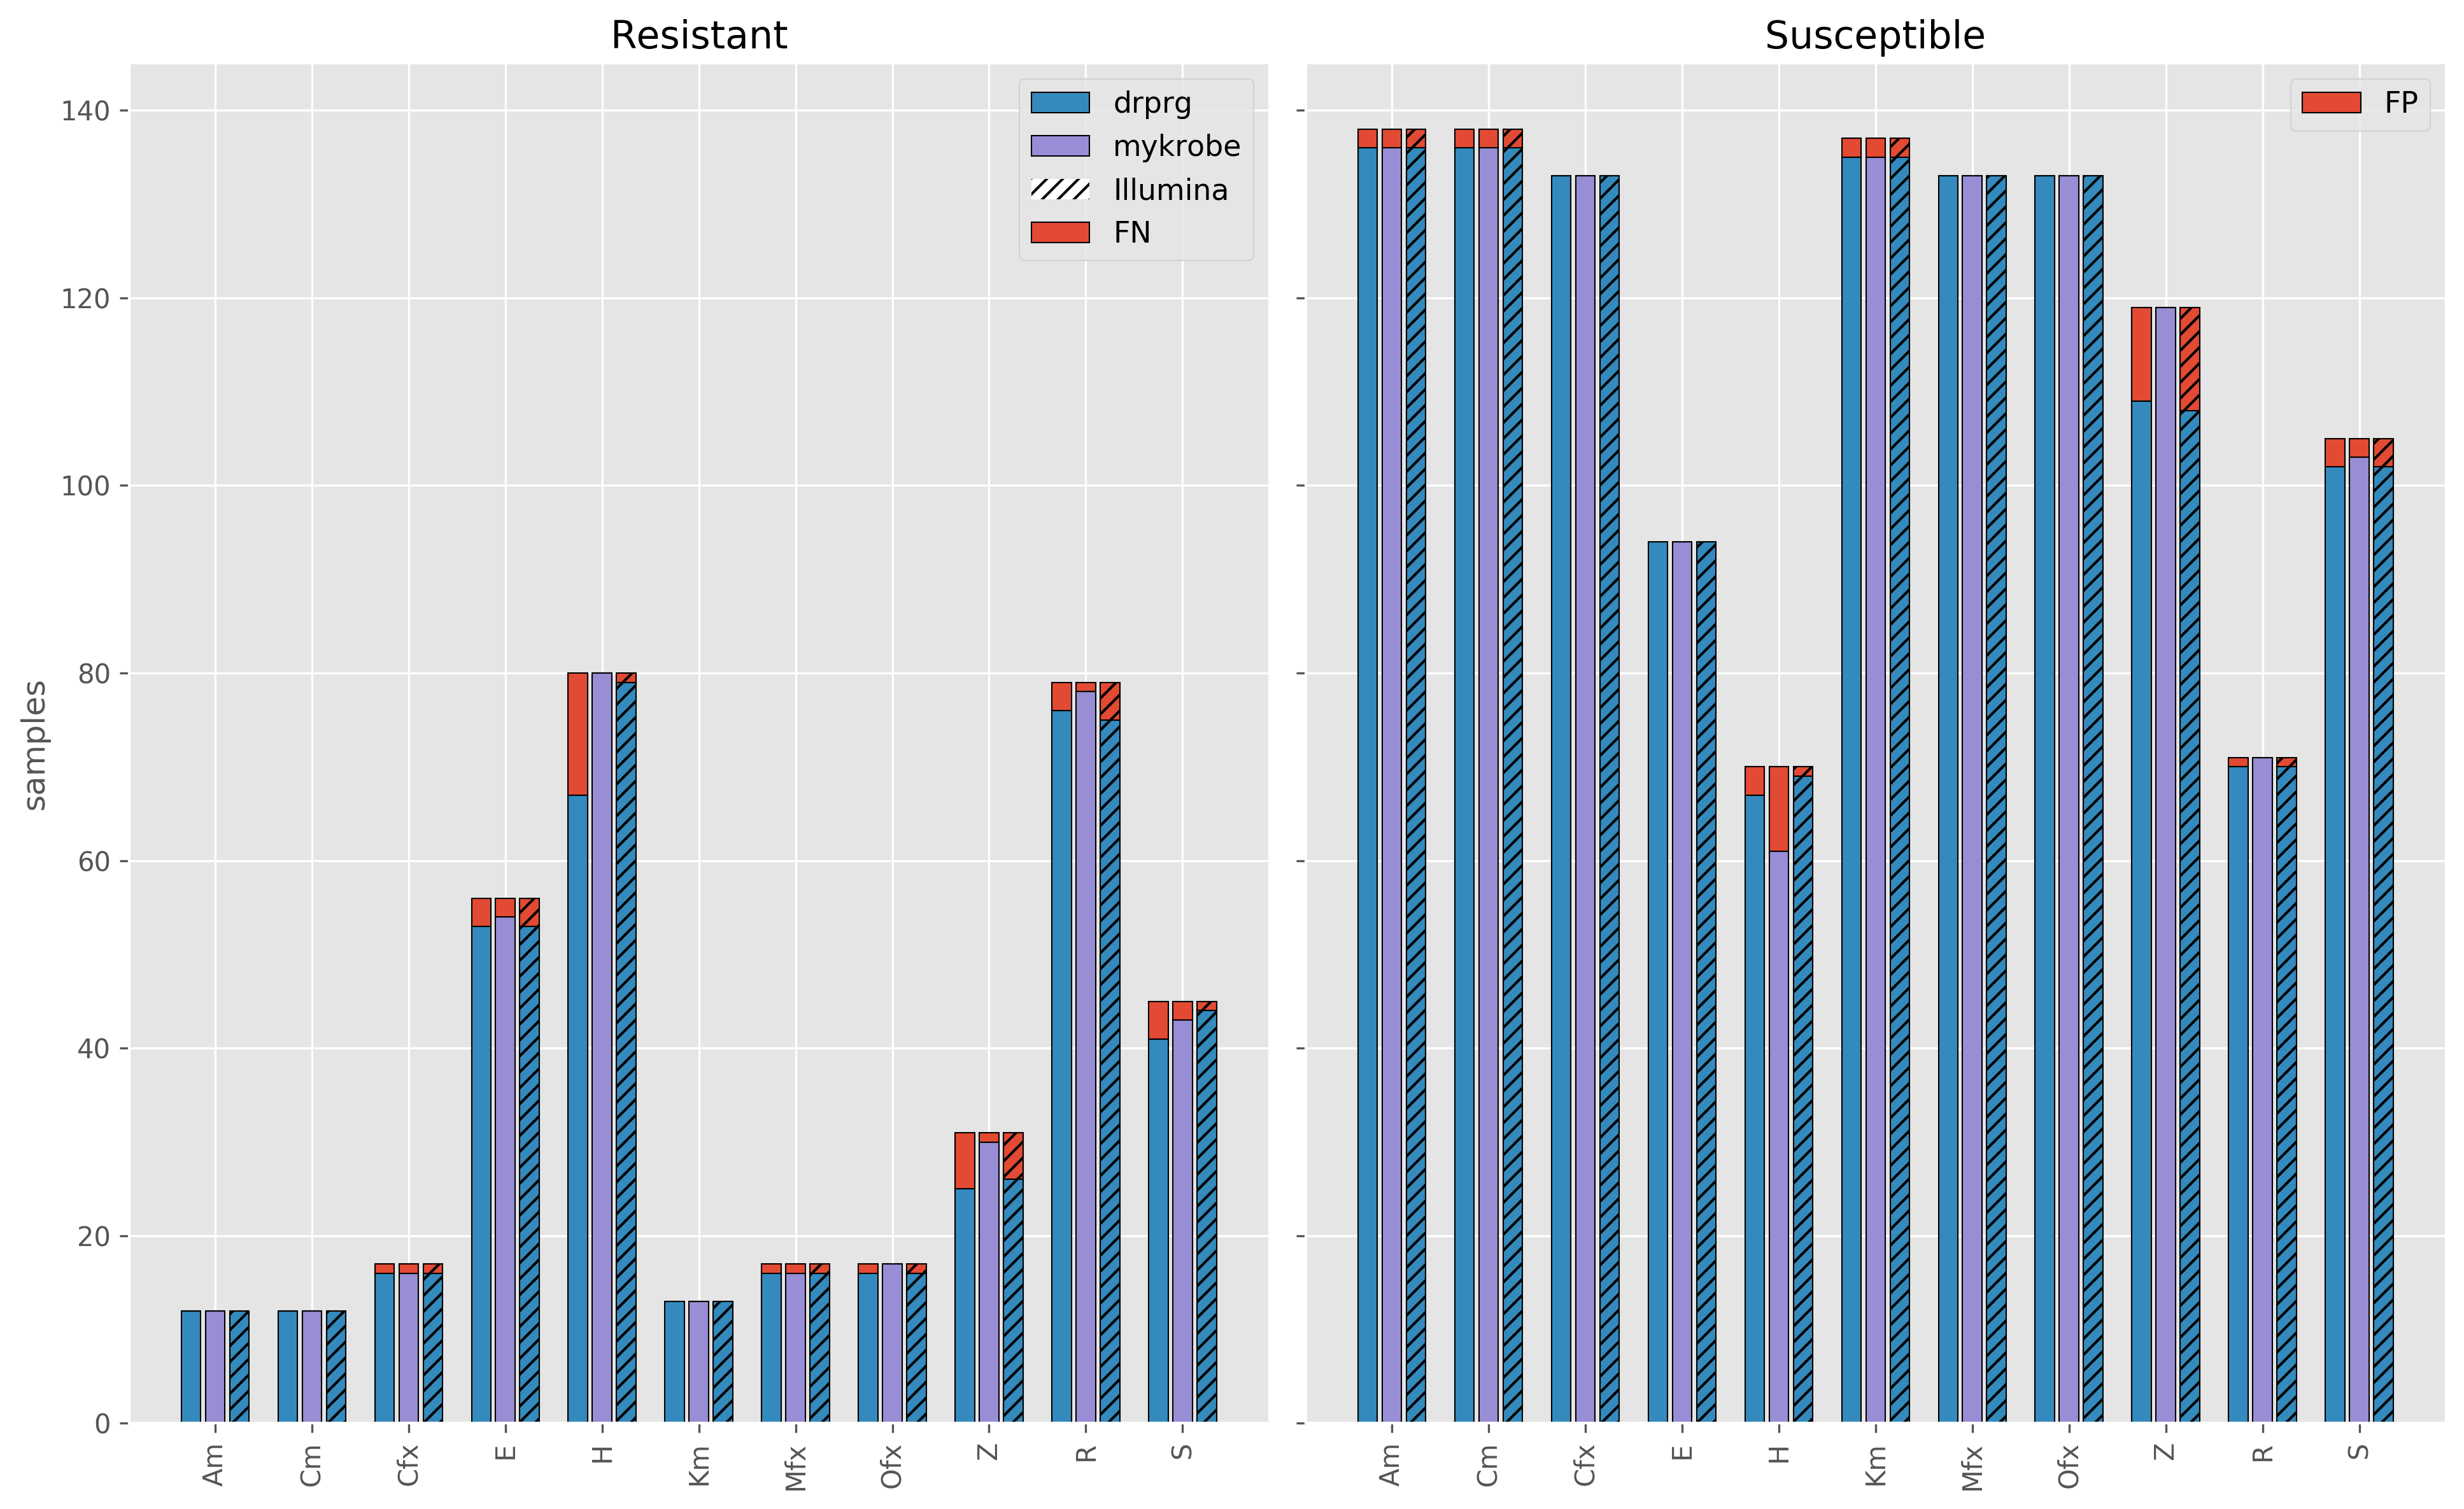
\includegraphics[width=0.90\columnwidth]{Chapter3/Figs/illumina_concordance.png}
\caption{{Number of resistant (left) and susceptible (right) genotypes correctly identified by mykrobe from Illumina (blue) and Nanopore (purple) data from the same samples. The genotypes are predictions from mykrobe with Illumina data. The red bars indicate missed (FN) or incorrect (FP) predictions. The x-axis shows the drugs with available phenotype data that mykrobe also makes predictions for. E - ethambutol; H - isoniazid; Z - pyrazinamide; R - rifampicin; S - streptomycin; Km - kanamycin; Am - amikacin; Ofx - ofloxacin; Cm - capreomycin; Mfx - moxifloxacin.
{\label{fig:geno-concordance}}
}}
\end{center}
\end{figure}

\begin{table}
\centering
\resizebox{\textwidth}{!}{%
\begin{tabular}{lllllllll}
\hline
Drug &
  Tool &
  Technology &
  FN(R) &
  FP(S) &
  FNR(95\% CI) &
  FPR(95\% CI) &
  PPV(95\% CI) &
  NPV(95\% CI) \\ \hline
\multirow{3}{*}{Amikacin} &
  \multirow{2}{*}{Drprg} &
  Illumina &
  0(12) &
  2(138) &
  0.0\% (0.0-24.2\%) &
  1.4\% (0.4-5.1\%) &
  85.7\% (60.1-96.0\%) &
  100.0\% (97.3-100.0\%) \\
 &
   &
  \multirow{2}{*}{Nanopore} &
  0(12) &
  2(138) &
  0.0\% (0.0-24.2\%) &
  1.4\% (0.4-5.1\%) &
  85.7\% (60.1-96.0\%) &
  100.0\% (97.3-100.0\%) \\
 &
  Mykrobe &
   &
  0(12) &
  2(138) &
  0.0\% (0.0-24.2\%) &
  1.4\% (0.4-5.1\%) &
  85.7\% (60.1-96.0\%) &
  100.0\% (97.3-100.0\%) \\
\multirow{3}{*}{Capreomycin} &
  \multirow{2}{*}{Drprg} &
  Illumina &
  0(12) &
  2(138) &
  0.0\% (0.0-24.2\%) &
  1.4\% (0.4-5.1\%) &
  85.7\% (60.1-96.0\%) &
  100.0\% (97.3-100.0\%) \\
 &
   &
  \multirow{2}{*}{Nanopore} &
  0(12) &
  2(138) &
  0.0\% (0.0-24.2\%) &
  1.4\% (0.4-5.1\%) &
  85.7\% (60.1-96.0\%) &
  100.0\% (97.3-100.0\%) \\
 &
  Mykrobe &
   &
  0(12) &
  2(138) &
  0.0\% (0.0-24.2\%) &
  1.4\% (0.4-5.1\%) &
  85.7\% (60.1-96.0\%) &
  100.0\% (97.3-100.0\%) \\
\multirow{3}{*}{Ciprofloxacin} &
  \multirow{2}{*}{Drprg} &
  Illumina &
  1(17) &
  0(133) &
  5.9\% (1.0-27.0\%) &
  0.0\% (0.0-2.8\%) &
  100.0\% (80.6-100.0\%) &
  99.3\% (95.9-99.9\%) \\
 &
   &
  \multirow{2}{*}{Nanopore} &
  1(17) &
  0(133) &
  5.9\% (1.0-27.0\%) &
  0.0\% (0.0-2.8\%) &
  100.0\% (80.6-100.0\%) &
  99.3\% (95.9-99.9\%) \\
 &
  Mykrobe &
   &
  1(17) &
  0(133) &
  5.9\% (1.0-27.0\%) &
  0.0\% (0.0-2.8\%) &
  100.0\% (80.6-100.0\%) &
  99.3\% (95.9-99.9\%) \\
\multirow{3}{*}{Ethambutol} &
  \multirow{2}{*}{Drprg} &
  Illumina &
  3(56) &
  0(94) &
  5.4\% (1.8-14.6\%) &
  0.0\% (0.0-3.9\%) &
  100.0\% (93.2-100.0\%) &
  96.9\% (91.3-98.9\%) \\
 &
   &
  \multirow{2}{*}{Nanopore} &
  3(56) &
  0(94) &
  5.4\% (1.8-14.6\%) &
  0.0\% (0.0-3.9\%) &
  100.0\% (93.2-100.0\%) &
  96.9\% (91.3-98.9\%) \\
 &
  Mykrobe &
   &
  2(56) &
  0(94) &
  3.6\% (1.0-12.1\%) &
  0.0\% (0.0-3.9\%) &
  100.0\% (93.4-100.0\%) &
  97.9\% (92.7-99.4\%) \\
\multirow{3}{*}{Isoniazid} &
  \multirow{2}{*}{Drprg} &
  Illumina &
  1(80) &
  1(70) &
  1.2\% (0.2-6.7\%) &
  1.4\% (0.3-7.7\%) &
  98.8\% (93.3-99.8\%) &
  98.6\% (92.3-99.7\%) \\
 &
   &
  \multirow{2}{*}{Nanopore} &
  13(80) &
  3(70) &
  16.2\% (9.7-25.8\%) &
  4.3\% (1.5-11.9\%) &
  95.7\% (88.1-98.5\%) &
  83.8\% (74.2-90.3\%) \\
 &
  Mykrobe &
   &
  0(80) &
  9(70) &
  0.0\% (0.0-4.6\%) &
  12.9\% (6.9-22.7\%) &
  89.9\% (81.9-94.6\%) &
  100.0\% (94.1-100.0\%) \\
\multirow{3}{*}{Kanamycin} &
  \multirow{2}{*}{Drprg} &
  Illumina &
  0(13) &
  2(137) &
  0.0\% (0.0-22.8\%) &
  1.5\% (0.4-5.2\%) &
  86.7\% (62.1-96.3\%) &
  100.0\% (97.2-100.0\%) \\
 &
   &
  \multirow{2}{*}{Nanopore} &
  0(13) &
  2(137) &
  0.0\% (0.0-22.8\%) &
  1.5\% (0.4-5.2\%) &
  86.7\% (62.1-96.3\%) &
  100.0\% (97.2-100.0\%) \\
 &
  Mykrobe &
   &
  0(13) &
  2(137) &
  0.0\% (0.0-22.8\%) &
  1.5\% (0.4-5.2\%) &
  86.7\% (62.1-96.3\%) &
  100.0\% (97.2-100.0\%) \\
\multirow{3}{*}{Moxifloxacin} &
  \multirow{2}{*}{Drprg} &
  Illumina &
  1(17) &
  0(133) &
  5.9\% (1.0-27.0\%) &
  0.0\% (0.0-2.8\%) &
  100.0\% (80.6-100.0\%) &
  99.3\% (95.9-99.9\%) \\
 &
   &
  \multirow{2}{*}{Nanopore} &
  1(17) &
  0(133) &
  5.9\% (1.0-27.0\%) &
  0.0\% (0.0-2.8\%) &
  100.0\% (80.6-100.0\%) &
  99.3\% (95.9-99.9\%) \\
 &
  Mykrobe &
   &
  1(17) &
  0(133) &
  5.9\% (1.0-27.0\%) &
  0.0\% (0.0-2.8\%) &
  100.0\% (80.6-100.0\%) &
  99.3\% (95.9-99.9\%) \\
\multirow{3}{*}{Ofloxacin} &
  \multirow{2}{*}{Drprg} &
  Illumina &
  1(17) &
  0(133) &
  5.9\% (1.0-27.0\%) &
  0.0\% (0.0-2.8\%) &
  100.0\% (80.6-100.0\%) &
  99.3\% (95.9-99.9\%) \\
 &
   &
  \multirow{2}{*}{Nanopore} &
  1(17) &
  0(133) &
  5.9\% (1.0-27.0\%) &
  0.0\% (0.0-2.8\%) &
  100.0\% (80.6-100.0\%) &
  99.3\% (95.9-99.9\%) \\
 &
  Mykrobe &
   &
  0(17) &
  0(133) &
  0.0\% (0.0-18.4\%) &
  0.0\% (0.0-2.8\%) &
  100.0\% (81.6-100.0\%) &
  100.0\% (97.2-100.0\%) \\
\multirow{3}{*}{Pyrazinamide} &
  \multirow{2}{*}{Drprg} &
  Illumina &
  5(31) &
  11(119) &
  16.1\% (7.1-32.6\%) &
  9.2\% (5.2-15.8\%) &
  70.3\% (54.2-82.5\%) &
  95.6\% (90.1-98.1\%) \\
 &
   &
  \multirow{2}{*}{Nanopore} &
  6(31) &
  10(119) &
  19.4\% (9.2-36.3\%) &
  8.4\% (4.6-14.8\%) &
  71.4\% (54.9-83.7\%) &
  94.8\% (89.1-97.6\%) \\
 &
  Mykrobe &
   &
  1(31) &
  0(119) &
  3.2\% (0.6-16.2\%) &
  0.0\% (0.0-3.1\%) &
  100.0\% (88.6-100.0\%) &
  99.2\% (95.4-99.9\%) \\
\multirow{3}{*}{Rifampicin} &
  \multirow{2}{*}{Drprg} &
  Illumina &
  4(79) &
  1(71) &
  5.1\% (2.0-12.3\%) &
  1.4\% (0.2-7.6\%) &
  98.7\% (92.9-99.8\%) &
  94.6\% (86.9-97.9\%) \\
 &
   &
  \multirow{2}{*}{Nanopore} &
  3(79) &
  1(71) &
  3.8\% (1.3-10.6\%) &
  1.4\% (0.2-7.6\%) &
  98.7\% (93.0-99.8\%) &
  95.9\% (88.6-98.6\%) \\
 &
  Mykrobe &
   &
  1(79) &
  0(71) &
  1.3\% (0.2-6.8\%) &
  0.0\% (0.0-5.1\%) &
  100.0\% (95.3-100.0\%) &
  98.6\% (92.5-99.8\%) \\
\multirow{3}{*}{Streptomycin} &
  \multirow{2}{*}{Drprg} &
  Illumina &
  1(45) &
  3(105) &
  2.2\% (0.4-11.6\%) &
  2.9\% (1.0-8.1\%) &
  93.6\% (82.8-97.8\%) &
  99.0\% (94.7-99.8\%) \\
 &
   &
  \multirow{2}{*}{Nanopore} &
  4(45) &
  3(105) &
  8.9\% (3.5-20.7\%) &
  2.9\% (1.0-8.1\%) &
  93.2\% (81.8-97.7\%) &
  96.2\% (90.7-98.5\%) \\
 &
  Mykrobe &
   &
  2(45) &
  2(105) &
  4.4\% (1.2-14.8\%) &
  1.9\% (0.5-6.7\%) &
  95.6\% (85.2-98.8\%) &
  98.1\% (93.3-99.5\%) \\ \cline{2-2} \cline{4-9} 
\end{tabular}%
}
\caption{Comparison of Nanopore drug resistance predictions with Illumina predictions.
For this comparison, we assume the mykrobe resistance prediction from Illumina data is correct and evaluate the Nanopore prediction accordingly.
FN=false negative; R=number of resistant samples; FP=false positive; S=number of susceptible samples; FNR=false negative rate; FPR=false positive rate; PPV=positive predictive value; NPV=negative predictive value; CI=Wilson score confidence interval}
\label{tab:geno-concordance}
\end{table}

%=========================================================================
\section{Effect of coverage on predictions}

% ***************
% text from authorea
It has previously been shown that deep coverage is required of Nanopore to accurately predict drug resistance (Votintseva 2017). As Nanopore sequencing advances quickly, and our dataset contains a broad depth-of-coverage range (~29-150x) we explore whether this requirement of high coverage still holds.
We binned samples into groups based on their read depth and looked at whether there is a higher proportion of errors in the lower coverage bins. Figure 9 shows there is no relationship between coverage and errors. Further work at depths lower than 30x is warranted, but there is convincing evidence here that samples with "only" 30x coverage should still yield reliable resistance predictions. 
% ***************

\begin{figure}
\begin{center}
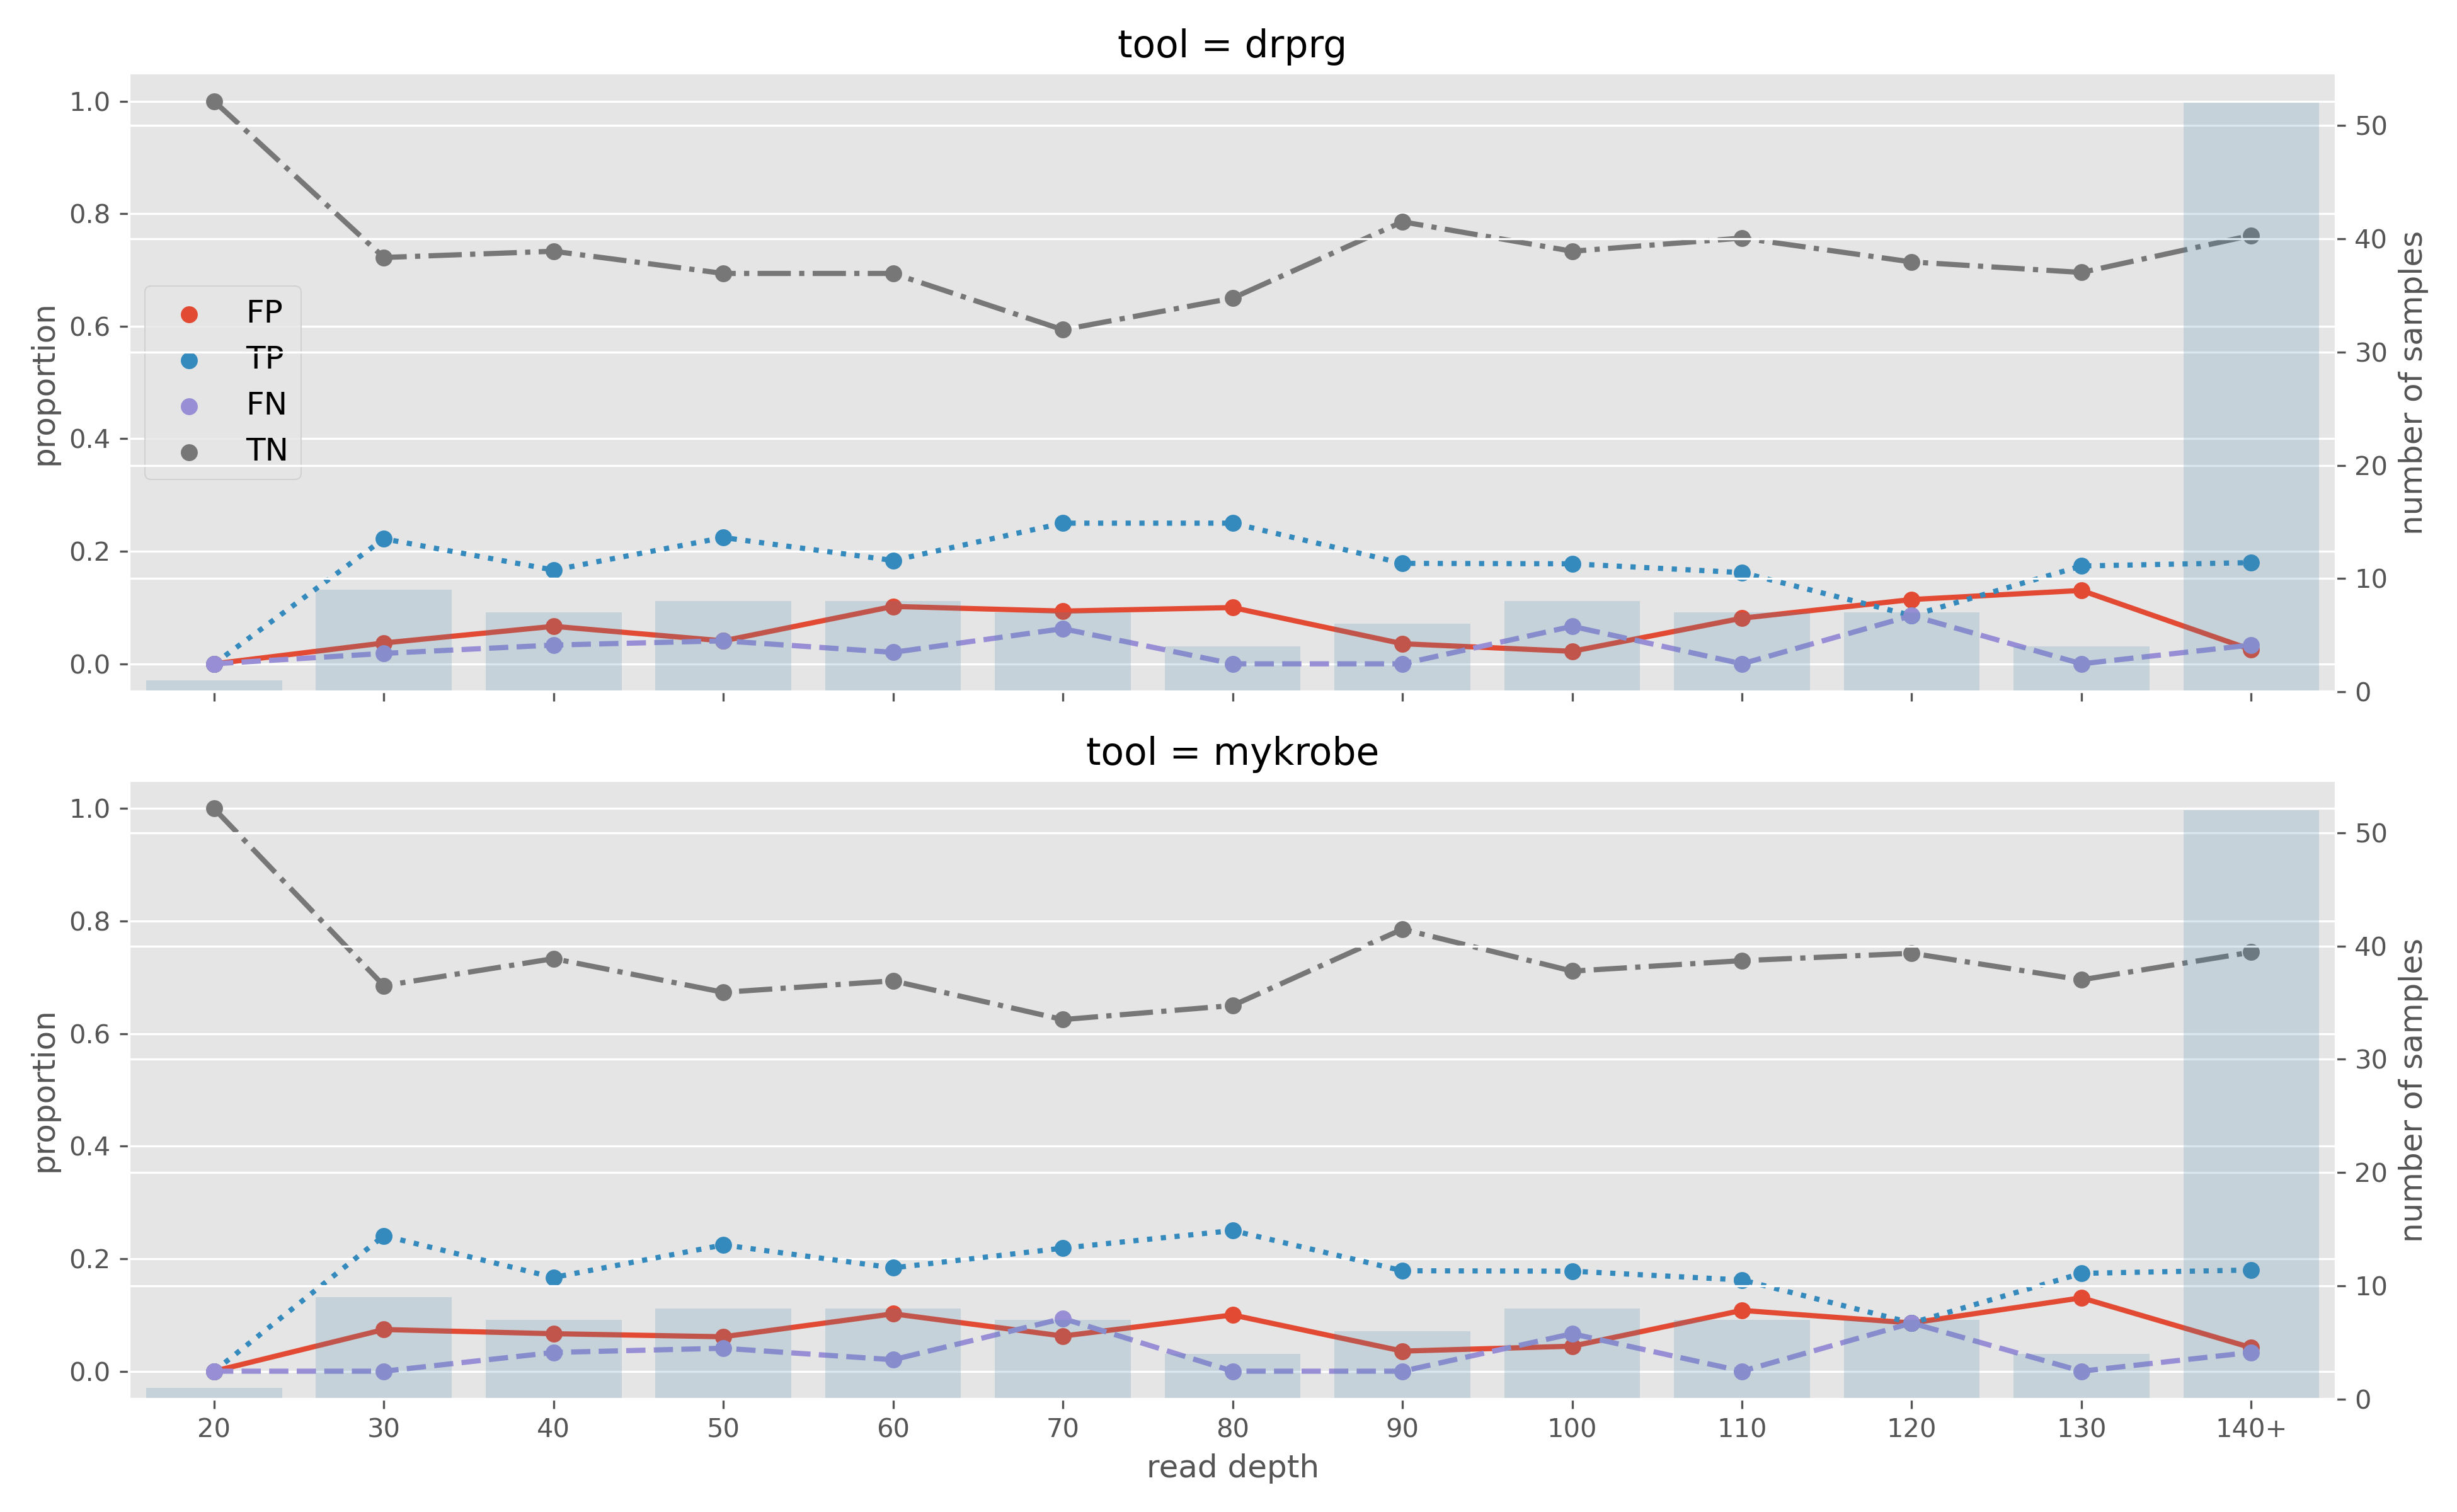
\includegraphics[width=0.90\columnwidth]{Chapter3/Figs/phenotype_coverage.png}
\caption{{Effect of Nanopore read depth on drprg (top) and mykrobe (bottom) phenotype prediction. Each point indicates the proportion (y-axis) of classifications of that type at the read depth (x-axis). Read depth is "binned". That is, read depth 40 is all samples with a read depth greater than 40 and less than or equal to 50. FP - false positive; TN - true negative; etc.
{\label{fig:pheno-covg}}
}}
\end{center}
\end{figure}
%=========================================================================
\section{Flagging novel variants not in panel}
\label{sec:drprg-discover}
%  what impact does this have on previous results
% http://www.crypticproject.org/wp-content/uploads/2018/09/Prediction-of-Susceptibility-to-First-Line-Tuberculosis-Drugs-by-DNA-Sequencing.pdf
% i guess what might be important here is whether FNs on phenotype are "fixed" by finding novel variants. Look through compass and bcftools VCFs for SNPs not in the panel
% we could also remove some common variants from the panel and see what difference novel would have then
% https://pubmed.ncbi.nlm.nih.gov/27436385/ shows lots of unknown mutations in gid, which we have a lot of novel variants for

%=========================================================================
\section{Discussion}
% The WHO target product profiles for new molecular assays for M. tuberculosis require more than 90% sensitivity and 95% specificity.7 from http://www.crypticproject.org/wp-content/uploads/2018/09/Prediction-of-Susceptibility-to-First-Line-Tuberculosis-Drugs-by-DNA-Sequencing.pdf
%=========================================================================
\section{Conclusion}

%=========================================================================
\section{Future work}

%=========================================================================
\section{Availability of data and materials}